% Template for ICASSP-2018 paper; to be used with:
%          spconf.sty  - ICASSP/ICIP LaTeX style file, and
%          IEEEbib.bst - IEEE bibliography style file.
% --------------------------------------------------------------------------
\documentclass{article}
\usepackage{spconf,amsmath,graphicx,hyperref}
\usepackage{caption,subfigure}

% Example definitions.
% --------------------
\def\x{{\mathbf x}}
\def\L{{\cal L}}

% Title.
% ------
\title{AUTHOR GUIDELINES FOR ICASSP 2018 PROCEEDINGS MANUSCRIPTS}
%
% Single address.
% ---------------
\name{Mattia Lecci, Federico Mason, Victor Cercos Llombart}
\address{UPC ETSETB - MET}
%
% For example:
% ------------
%\address{School\\
%	Department\\
%	Address}
%
% Two addresses (uncomment and modify for two-address case).
% ----------------------------------------------------------
%\twoauthors
%  {A. Author-one, B. Author-two\sthanks{Thanks to XYZ agency for funding.}}
%	{School A-B\\
%	Department A-B\\
%	Address A-B}
%  {C. Author-three, D. Author-four\sthanks{The fourth author performed the work
%	while at ...}}
%	{School C-D\\
%	Department C-D\\
%	Address C-D}
%
\begin{document}
%\ninept
%
\maketitle


\begin{abstract}
%
In this report we try to perform chord recognition, meaning the extraction of the name of a musical chord from an audio file. After describing the techniques used, we show the performance obtained in two different scenarios: the first one is a simple single-chord single-instrument kind of scenario, while the second one considers full songs.

Through the implementation of classical \textit{Machine Learning} (ML) techniques and \textit{Hidden Markov Models} (HMM) we illustrate the difficulties and show advantages of fairly complicated algorithms over the simple ones.
%
\end{abstract}
\section{Introduction}
\label{sec:intro}

A chord is defined as two or more notes sounding simultaneously	.(1) This is normally achieved by playing the different notes that form the chor at the same time, in other cases like arpeggios and broken chords, the notes are played separated and successively. (FOTO¿??) The harmonic content of a music piece is defined by the chords and the progressions of them. This aspect is very important to understand and analyse tonal music.(2) This is an important applications in cover songs identification where the harmonic analysis is more robust. (3)  The chord names vary depending on the number of notes that form them: "Triad","Seventh", "Ninth",... The most commonly used chords in music pieces are the "triads", in which this project focusses. This kind of chord is composed by three different notes. To avoid problems with the different octaves and their pitch, "chromas" are used instead of distinct notes.(4) \\(Foto) The notes of a chord are selected according to the musical distance between pitches of simoultaneously sounding notes, the so called musical interval. The chords are commonly classified as "minor", "major", "dimished" and "augmented". This project focusses on minor and major chords. The name of the chord is driven from the root note of it, usally this note is the lowest one. Taking the triad as an example the second note is called third, because it's the third chroma from the root note on, so the last note is called fifth. In the minor triad only the 2 noe changes, to a minor third interval. Some chords present inversions, where the root note is not in the lowest position.
\section{Techniques used}
\label{sec:techniques}

\subsection{Mel-frequency Cepstral Coefficients (MFCC)}
\label{subsec:mfcc}


\subsection{Template-based chord recognition}
\label{subsec:templates}

Template matching consists of two steps: first, the templates are computed and second, the distance between the extracted features and the templates is calculated. In this project two types of templates are used: the \textit{binary templates} and the \textit{harmonic templates}. Binary templates are a simple binary representation of the chords (0 if the note is not present, $1/\sqrt{3}$ if the note is present). In order to create more accurate templates, the harmonics of each chord's note are also taken in count for the harmonic templates.

Adopting techniques taken from \cite{gomez2006tonal},\cite{oudre2009chord}, the first 6 harmonics of each note where used, exponentially attenuating each successive harmonic of each note (i.e. multiplying the harmonics by $[1, s, s^2, s^3, s^4, s^5]$, with the suggested factor $s=0.6$) and finally adding everything up and normalizing the result.
\subsection{Gaussian Mixture Models (GMMs)}
\label{subsec:gmm}

\textit{Gaussian Mixture Models} are a statistic technique used to identify classes within an overall population. At the end of the process, each class is assigned to a \textit{Multivariate Gaussian Distribution} (MGD).  As widely known, MGDs are defined only through its \textit{mean vector} and a \textit{covariance matrix}. We notice that given a MGD, it is very simple to evaluate the probability distribution function for that point. We just need to implement the \textit{Mahalanobis distance} which measures how many standard deviations the selected object is far from the distribution mean, taking into account the covariance matrix. \\
%
MATLAB defines a class called \texttt{gmdistribution} which allows you to easily create an object which contains one or more MGDs. MATLAB also offers the method \texttt{mahal} to compute the Mahalanobis distance between an object $X$ and a GMM. \\
\subsection{Multiclass Support Vector Machines (MC-SVM)}
\label{subsec:svm}

\textit{Support Vector Machines} (SVM) are a well known and widely used \textit{Machine Learning} algorithm for binary classification. Before Neural Networks became so popular, they generally outperformed most of the other standard classification (and also regression) algorithms. Some good advantages over them is the possibility of choosing non-linear kernels (the most famous ones are the \textit{Gaussian/RBF} and the \textit{Polynomial}). Also, they are far easier to program and optimize than Neural Networks (less hyperparameters) and they tend to overfit less.\\
%
Their main problem, though, is that they were conceived for binary classification. Their extension to multiclass classification is not trivial but there are some standards ways to do it. One of them is already implemented in Matlab and it's called \textit{Error-Correcting Output Codes} (ECOC). It works by creating multiple classifiers and assigning to each of them some classes to be considered positive and some other to be negative and by assigning weights to these binary classifiers, the final decision is taken.\\
%
For our tests we used the \textit{One-vs-One} method, meaning that we create a classifier for every couple of classes ($O(K^2)$) assigning one to the positive and one to the negative, while ignoring everything else. This is usually a good tradeoff between complexity and precision, but other options could be explored in future works.
\subsection{Hidden Markov Models (HMMs)}
\label{subsec:hmm}

\textit{Hidden Markov Models} are an extremely powerful technique that has been widely used in speech recognition application for twenty years. A HMM consistis in an extension of the classical Markov Model scenario, in which observations are considered probabilistic functions of states. The final result is a pair of stochastic processes connected to each other; one process is directly observable, the other process is not and therefore is called "hidden". A more detailed theory about HMM working can be found in \cite{LawrenceHMMtutorial}. \\
%
In the speech recognition field, HMMs are used as statistical method in order to recover specific sequences of sound. The validity of HMMs in the the particular case of chords transcription has already been demostrated several times, as in \cite{AlexDanEMplusHMM} and \cite{belpickMusic}. Both of these works use the HMM approach proposed in \cite{GoldMorganSpeechRecogn}, training HMM with the \textit{expectation-maximization algorithm}. As our work is not limited to implementing HMM, we decided to combine HMM with the SVM technique previously presented. \\
%
As suggested in \cite{GoldMorganSpeechRecogn}, the \textit{Viterbi algorithm} is an efficient way of working with HMMs. Given a HMM scenario and a sequence of observations, Viterbi's algorithm aims to find the most likely sequence of states. Given a total number of states $N$ and a sequence of $T$ observations, the Viterbi algorithm has a complexity equal to $O(TN^2)$. In our work the implementation of Viterbi's algorithm represented one of the most difficult challenges. Already existing code \cite{MatlabViterbi} raised problems and therefore it needed to be carefully adapted to the experiment setup.

\section{Experiment Setup}
\label{sec:setup}

Our experimentation was split in two parts: the first was about recognizing a single chord from a single chord track, the second one was about recognizing the chords of full songs.\\
%
For the first part, we used the dataset \texttt{jim2012Chords} \cite{jim2012Chords} created for their paper \cite{JimChordsPaper}. It's composed of a total of over $2.000$ recordings of 10 guitar chords (both major and minor triads). Four different Guitars are used, as well as Piano, Violin and Accordion. Some tracks were recorded in an anechoic chamber, some other in a noisy environment. For each one of the tracks we obtain a 12-dimensional feature vector using \textit{Chroma Toolbox} and taking the maximum value for each note. Looking at Fig.~\ref{fig:CENSexample}, the idea is that we are interested in high values of specific groups of notes in order to guess the chord and the maximum value is a simple way of doing this. It's biggest disadvantage is that impulsive noisy environment can easily mask the useful information introducing high values in the wrong notes. Finally, we run the different methods on these obtained 12D vectors.\\
%
Fo the second part, we used \textit{The Beatles}' discography, which has been professionally transcribed. \dots
\section{Results}
\label{sec:results}


\begin{figure} [h!]
	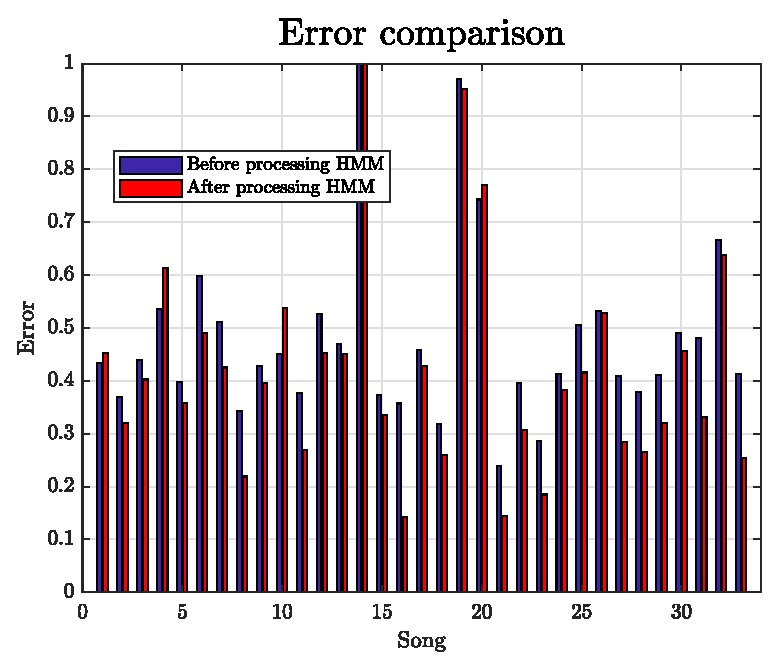
\includegraphics[width=0.5\textwidth]{img/Result_HMM/CENS/plot03071}
	\caption{Error comparison using CENS features (train = 0.8; test = 0.2)}
\end{figure}


\begin{figure} [h!]
	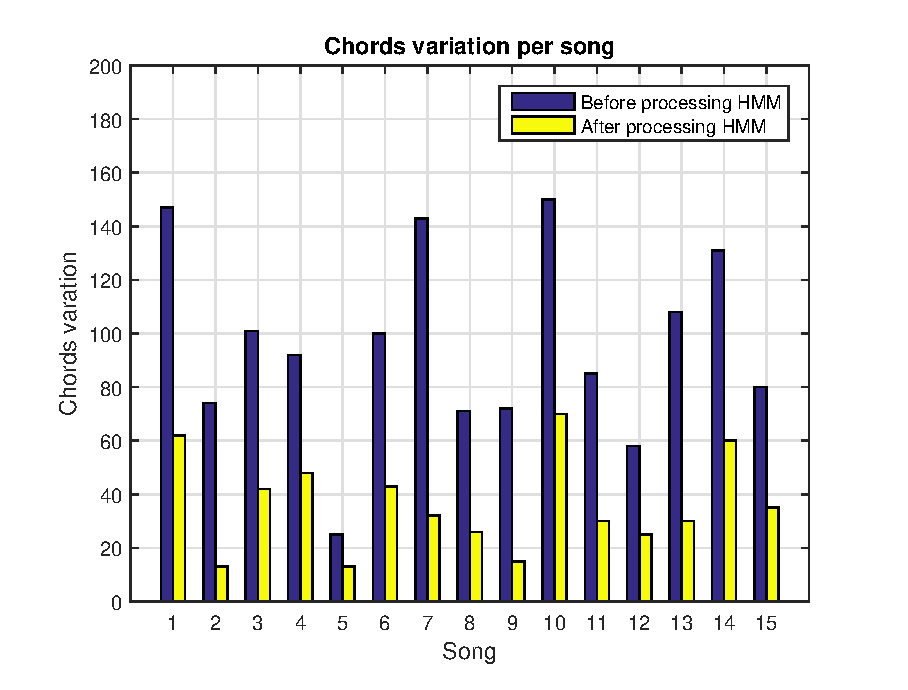
\includegraphics[width=0.5\textwidth]{img/Result_HMM/SMOOTHING/smoothingPerSong0109}
	\caption{Chords variation per song using CENS features (train = 0.9; test = 0.1)}
\end{figure}

\begin{figure} [h!]
	\includegraphics[width=0.5\textwidth]{img/Result_HMM/SMOOTHING/smoothingSingleSong0109}
	\caption{Chord variation in a single song using CENS features (train = 0.9; test = 0.1)}
\end{figure}

\section{Conclusions}
\label{sec:conclusions}

After seeing the results in Sec.~\ref{sec:results}, it should be clear that the more advanced techniques described in Sec.~\ref{sec:techniques} improve the results very significantly over the oldest and simplest ones.

In particular, CENS features are able to perform really well with all classifiers but the most advanced ones (SVM with non-linear kernels) clearly outperform all the others.

Using this information, we tried to predict chords in full songs having, of course, poorer results, due to the increased complexity of the problem. The HMM-based approach, again, was able to improve performance over the trivial \textit{per-frame} one.

Future works might try to use different type of features and classifiers for the general chord recognition problem. When dealing with entire songs, instead, it might be useful to either extract or subtract specific instruments (e.g. drums) and voice, since we believe they are the main cause of the high error rates obtained.

% References should be produced using the bibtex program from suitable
% BiBTeX files (here: strings, refs, manuals). The IEEEbib.bst bibliography
% style file from IEEE produces unsorted bibliography list.
% -------------------------------------------------------------------------
\bibliographystyle{IEEEbib}
\bibliography{bibliography}

\end{document}
